\subsection{\large{Python IDE}}
Ihr sitzt jetzt vor dem PC und wollt ein paar Schritte in der Programmiersprache Python gehen. Wir haben uns gedacht, dass wir die Gelegenheit nutzen ein paar Pixel auf die Matrix zu zaubern. Da das als Gruppe vielleicht mehr Spaß macht, können alle gleichzeitig ihre Pixel setzen. Und damit nicht alle Pixel einzeln gesetzt werden, lernen wir wie uns der Computer dabei hilft.\\
Mit einer Python Entwicklungsumgebung (IDE) können wir einfach unsere Python Programme schreiben.\\ Für Linux gibt es z.B. Thonny.\\
\subsection{\large{PixelMatrix}}
Die Bibliothek ,,PixelMatrix`` macht alles, was man im Moment zum Pixeln noch nicht wissen muss. Also halten wir uns erst einmal daran. Das Einzige was wir wissen müssen, ist die IP-Adresse von der Matrix. Diese speichern wir in der Variable HOST.\\
\begin{lstlisting}[language=Python, caption=Bibliotheken]
import PixelMatrix
from time import sleep
from random import random

HOST = "192.168.    .    "    # gopixelflut Server 
\end{lstlisting}
%192.168.1.226
mit \textbf{import} sagen wir, dass wir diese Programmfetzen vom WAK-Lab benutzen wollen. Außerdem wurde die Zeit erfunden und von der benutzen wir den Schlaf und außerdem den Zufall. Damit lässt sich nachher einiges steuern.
\subsection{\large{Farben}}
\begin{lstlisting}[language=Python, caption=Farben]
Weiss = (255, 255, 255)
Rot   = (255, 0, 0)
Gruen = (0, 255, 0)
Blau  = (0, 0, 255)
Schwarz  = (0,0,0)
Lila  = (200,100,200)
Rosa  = (255,0,132)
\end{lstlisting}
Hier geben wir die Helligkeit der einzelnen Farbtöne an. In Klammern erst Rot, dann Grün dann Blau. Die Angaben sind im Bereich von 0 bis 255 von dunkel bis hell. Damit ist Rot z.B. (255, 0, 0). Wer möchte kann seine Farbe googlen: ,,Farbcode Rosa``.\\
\begin{minipage}[t]{\textwidth}
  \centering
  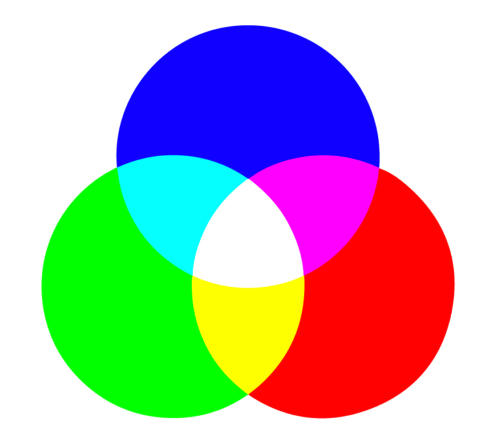
\includegraphics[width=0.42\textwidth]{pictures/RGB.png}
  \captionof{figure}{RGB Farbraum}
  \label{img:RGB}
\end{minipage}

\subsection{\large{Das Matrix Objekt}}
Man spricht von Objekt wenn so ein Ding baut, was Dinge tun kann. Ich hätte ihm auch einen anderen Namen geben können, aber nun heist es Matrix. \\
%Das kann man sich so vorstellen, dass man wenn man nun im %Katalog ein schönes Buch gesehen hat, dann kaufen wir uns das jetzt auch und nennen es Matrix.\\
\begin{lstlisting}[language=Python, caption=Das Matrix Objekt]
Matrix = PixelMatrix.PixelMatrix(HOST)
\end{lstlisting}
Matrix kann nun alles was wir aus der Bibliothek PixelMatrix verwenden wollen. Zwischen den Namen und dem was wir tun wollen setzen wir einen Punkt z.B. Matrix.PutPixel(x,y) .\\
Das WAK-Lab hat schon man ein paar Funktionen gebaut, damit wir gleich loslegen können.\\
\begin{lstlisting}[language=Python, caption=Matrix Löschen]
Matrix.White()
\end{lstlisting}
Das können wir gleich einmal ausprobieren. Dafür Starten wir das Python Programm mit F5.\\
\ \\
Matrix.White() oder Matrix.Black() Schaltet alle LEDs an oder aus. Da wir ja als Team arbeiten wollen, wäre es nicht nett allen andern die Pixel zu löschen also schreiben wir eine Raute \# vor den Befehl und Kommentieren ihn dadurch aus (er wird also nicht mehr ausgeführt). Sowieso können wir die Raute \# benutzen um uns einige Kommentare aufzuschreiben, damit wir noch wissen was wir gerade mit dem Programm wollten.\\
\begin{lstlisting}[language=Python, caption=Einen Pixel setzen]
#Hier wird ein Pixel gesetzt
Matrix.Putpixel(1,1, Rot)
\end{lstlisting}
Setzt eine Pixel oben Links in der Ecke. Dort fangen wir an zu Zählen mit 1,1. Die Matrix hat 60x33 Punkte, ihr könnt also auch mit: \begin{lstlisting}[language=Python, caption=Noch einen Pixel setzen]
Matrix.Putpixel(60,33, Rot)
\end{lstlisting}
unten rechts einen Punkt setzen.\\
\subsection{\large{Einen Befehl mehrmals ausführen}}
Um einen Befehl mehrmals auszuführen brauchen wir eine Schleife. Dafür nehmen wir den Befehl ,,for``.
\begin{lstlisting}[language=Python, caption=For Schleifen]
for i in range(10,20):
	Matrix.Putpixel(i,10,Rot)
\end{lstlisting}
In Python benutzt man die Tabulatortaste um einen Befehl einzurücken der innerhalb der Schleife mehrmals ausgeführt wird. Die Angabe range(10,20) lässt i von 10 bis 19 durchzählen, und nun setzen wir damit 10 Punkte von x=10..19 und y=10. \\
\ \\
Damit man eine Punkt auch wieder löschen könnt, malen wir einfach einen schwarzen Punkt und zwar 3 Pixel hinter dem Roten. Damit es nicht zu schnell geht warten wir kurz 0,5 Sekunden:
\begin{lstlisting}[language=Python, caption=For Schleifen]
for i in range(10,20):
	Matrix.Putpixel(i,10,Rot)
	Matrix.Putpixel(i-3,10,Schwarz)
	sleep(0.5)
\end{lstlisting}

\subsection{\large{Wir malen ein Bild}}
Natürlich haben wir auch vorbereitet, dass man ein Bild an die Matrix projizieren kann. Dafür gibt es die Picture() und die AnimateGif() Funktionen. Wenn wir also ein kleines Bild in das Verzeichnis legen, können wir es laden und anzeigen.
\begin{lstlisting}[language=Python, caption=Ein Bild]
Matrix.Picture("NeueWelten.png", 10,0)
\end{lstlisting}
oder:
\begin{lstlisting}[language=Python, caption=Ein Animiertes Gif]
Matrix.AnimateGif("NeueWelten.gif", 10,0)
\end{lstlisting}
\begin{minipage}[t]{\textwidth}
  \centering
  
\includegraphics[width=0.9\textwidth]{pictures/NW.png}
  \captionof{figure}{Neue Welten Logo}
  \label{img:NW}
\end{minipage}
\subsection{\large{Einige Hilfen}}
\begin{lstlisting}[language=Python, caption=Mathematik]
A = 1+1
B = A*2
\end{lstlisting}
\begin{lstlisting}[language=Python, caption=Eine verschachtelte Schleife]
for x in range(1,60):
	for y in range(1,30):
		Matrix.Putpixel(x,y,Gruen)
\end{lstlisting}
\begin{lstlisting}[language=Python, caption=Eine bedingte Abarbeitung]
if x>y:
	Matrix.Putpixel(x,y,Gruen)
else:
	Matrix.Putpixel(x,y,Blau)
	
if x==y:
	Matrix.Putpixel(x,y,Rot)
\end{lstlisting}
\begin{lstlisting}[language=Python, caption=Ein Zufallspunkt]
punkt = (60*random(),33*random())
\end{lstlisting}
\begin{lstlisting}[language=Python, caption=Eine Warteschlange]
queue = []
queue.append((x,y))
value = queue.pop(0)
\end{lstlisting}
%\newpage